\documentclass[a4paper, 14pt,russian]{extarticle}

\usepackage[russian]{babel}
\usepackage[T2A]{fontenc}
\usepackage[utf8]{inputenc}
%Соответствующий математический шрифт для Times new roman
\usepackage{newtxmath}
\usepackage{fontspec} 
\usepackage{multirow}
%\usepackage{polyglossia}
%Times new roman
\defaultfontfeatures{Ligatures={TeX},Renderer=Basic} 
\setmainfont[Ligatures={TeX,Historic}]{Times New Roman}
\setmainfont{Times New Roman}
\setsansfont{Arial}
\setmonofont{Courier New}
\newfontfamily\cyrillicfont[Script=Cyrillic]{Times New Roman}
\newfontfamily\cyrillicfontsf[Script=Cyrillic]{Arial}
\newfontfamily\cyrillicfonttt[Script=Cyrillic]{Courier New}

%\setdefaultlanguage{russian}

%Геометрия
\usepackage{geometry}
\geometry{top=20mm}
\geometry{bottom=15mm}
\geometry{left=20mm}
\geometry{right=15mm}
\usepackage{setspace}
%Нормальные дроби через запятую
\usepackage{ncccomma}

\newcommand{\changefont}{%
	\fontsize{12}{11}\selectfont
}

%Заголовки
\usepackage{fancyhdr}
%\pagestyle{fancy}
%\fancyhf{}
%\renewcommand{\sectionmark}[1]{\markright{#1}}
%\fancyhead[R]{\changefont \slshape \leftmark}
%\fancyhead[L]{\changefont \slshape \rightmark}
%\newcommand{\ssubsection}[1]{\subsection*{#1}
%	\addcontentsline{toc}{subsection}{#1}
%	\markright{#1}{}}
\cfoot{\thepage}

%\полуторный интервал
\setstretch{1.15}
\setlength{\parindent}{1.25cm}

\usepackage{amsmath, amsfonts, mathtools}
\usepackage{physics}
\usepackage{indentfirst}
\usepackage{xcolor}
\usepackage{alltt}
\usepackage{graphicx}
\usepackage{wrapfig}
\usepackage{pgfplots}
\usepackage{filecontents}

%Настройка ссылок
\usepackage{hyperref}
%\usepackage{upgreek}
%\renewcommand{\beta}{\upbeta}
\hypersetup{
	colorlinks,
	citecolor=black,
	filecolor=black,
	linkcolor=black,
	urlcolor=black
}
\usepackage{caption}
\usepackage{subcaption}
\renewcommand{\thesubfigure}{\asbuk{subfigure}}
\newcommand\scalemath[2]{\scalebox{#1}{\mbox{\ensuremath{\displaystyle #2}}}}
%\renewcommand{\thesection}{\Asbuk{section}}
\DeclareCaptionLabelSeparator{dot}{. }
\captionsetup{justification=centering,labelsep=dot}
\usepackage{titlesec}

%Формат заголовков
\titleformat{\section}{\bfseries\filcenter\Large}{\thesection}{1em}{}
\titleformat{\subsection}{\bfseries\filcenter\large}{\thesubsection}{1em}{}
\titleformat{\subsubsection}{\bfseries\filcenter\normalsize}{\thesubsubsection}{1em}{}

\usepackage{chngcntr}

%Включить в нумерацию картинок раздел
\counterwithin{figure}{section}

%Листинги кода и их стили
\usepackage{listings}
\usepackage{minted}
\lstdefinestyle{c++} {
	language=C++,
	breaklines=true,
	frame=single,
	numbers=left,
	basicstyle=\footnotesize\ttfamily,
	keywordstyle=\bfseries\color{green!40!black},
	commentstyle=\itshape\color{purple!40!black},
	identifierstyle=\color{blue},
	backgroundcolor=\color{gray!10!white},
}

\lstdefinestyle{python}{
	language=Python,
	breaklines=true,
	frame=single,
	numbers=left,
	keywordstyle=\bfseries\color{green!40!black},
	frame=lines,
	basicstyle=\footnotesize\rmfamily
}

\lstdefinestyle{cmd}{
	breaklines=true,
	frame=single,
	basicstyle=\footnotesize\ttfamily,
	frame=lines
	basicstyle=\footnotesize
}
\usepackage{tikz}
\usepackage{tkz-base}
\usetikzlibrary{quotes,angles}
\usetikzlibrary {arrows.meta}
%\usepackage{tkz-euclide}
\usetikzlibrary{calc}
\usetikzlibrary{shapes.geometric, shapes.misc, arrows}

\tikzstyle{startstop} = [rectangle, rounded corners, 
minimum width=3cm, 
minimum height=1cm,
text centered, 
draw=black]

\tikzstyle{io} = [trapezium, 
trapezium stretches=true, % A later addition
trapezium left angle=70, 
trapezium right angle=110, 
minimum width=3cm, 
minimum height=1cm, text centered, 
draw=black]

\tikzstyle{process} = [rectangle, 
minimum width=3cm, 
minimum height=1cm, 
text centered, 
text width=5cm, 
draw=black]

\tikzstyle{decision} = [diamond, 
minimum width=3cm, 
minimum height=1cm, 
text centered, 
draw=black]

\tikzstyle{startfor} = [chamfered rectangle, 
chamfered rectangle corners={north west, north east},
minimum width=3cm, 
minimum height=1cm, 
text centered, 
draw=black]

\tikzstyle{endfor} = [chamfered rectangle, 
chamfered rectangle corners={south west, south east},
minimum width=3cm, 
minimum height=1cm, 
text centered, 
draw=black]

\tikzstyle{block} = [style=draw, 
	minimum width = 1.6cm,
	minimum height = 1.2cm]
\tikzstyle{arrow} =[-{Latex[length=3mm]}, thick]

\newcommand{\drawsum}[2]{\node[draw,
	circle,
	minimum size=1cm
	] (#1) at #2{};
	\draw (#1.north east) -- (#1.south west)
	(#1.north west) -- (#1.south east)}

\newcommand{\fillsumsouth}[1]{\draw[fill=black] (#1.center) -- ++(-135:0.5cm) arc (-135:-45:0.5cm) -- cycle}
\newcommand{\fillsumnorth}[1]{\draw[fill=black] (#1.center) -- ++(135:0.5cm) arc (135:45:0.5cm) -- cycle}
\usepackage{pdfpages}
\usepackage{adjustbox}
\usepackage{array}
\usepackage{multirow}
\pgfplotsset{compat=1.18}
\usetikzlibrary{arrows.meta}
\usepackage[europeanresistors, americaninductors, straightvoltages]{circuitikz}

\begin{document}
	
	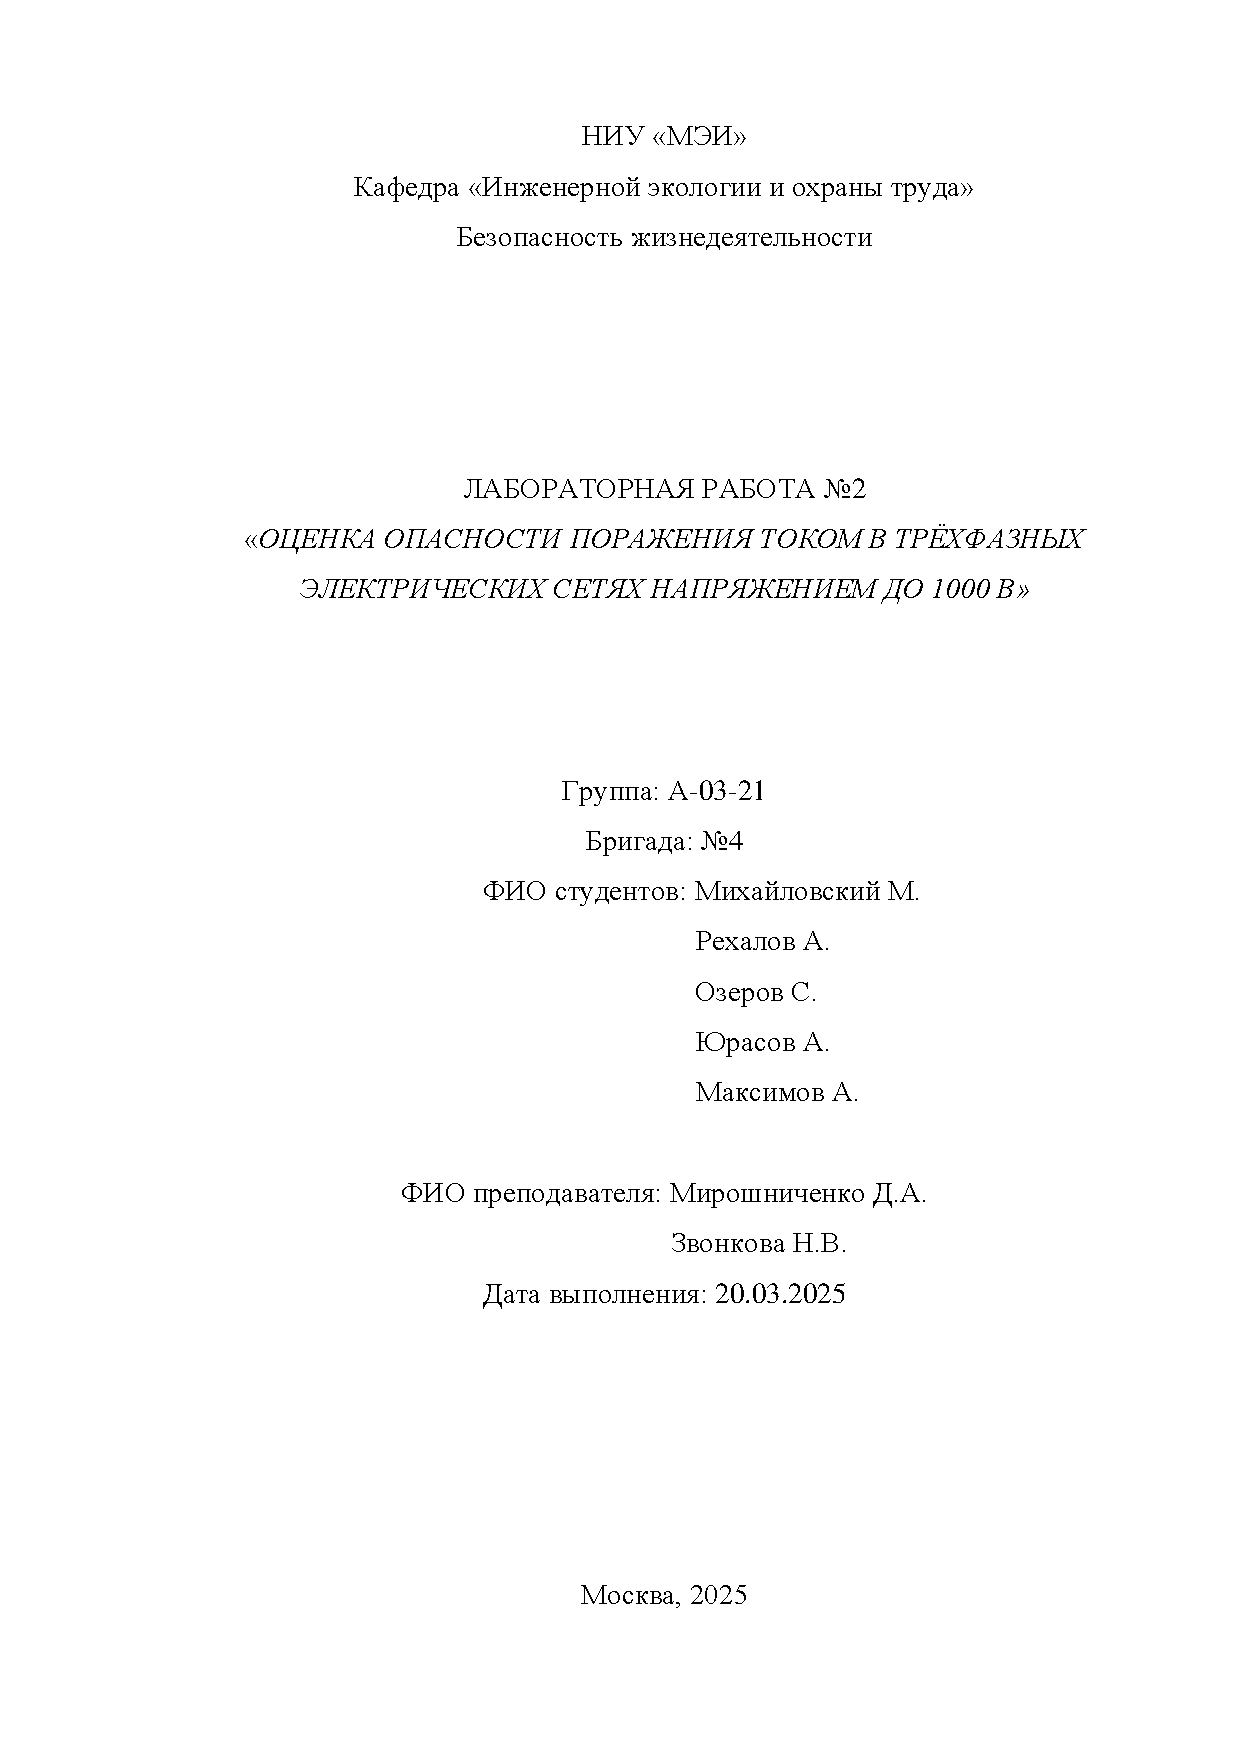
\includepdf[pages=-]{Титульник.pdf}
	\pagenumbering{arabic}
	\setcounter{page}{2}
	%\tableofcontents
	%\newpage
	
	\section*{Цель работы}
	
	Оценить опасность прикосновения человека к токоведущим частям
	трёхфазных сетей напряжением до 1000 В.
	
	Изучить	влияние	параметров сетей (режима нейтрали, сопротивлений изоляции и ёмкости фазных проводников относительно земли) на опасность поражения человека электрическим током.
	
	\section{Оценка опасности прямого прикосновения к токоведущими частям}
	
	В ходе работы были проведены измерения тока, протекающего через тело человека, при прикосновении к токоведущим частям трёхфазной линии с фазным напряжением 220\,В. Результаты измерений для разных типов сетей и прикосновений к различным проводам приведены в таблице \ref{table_currents}.
	
	Сопротивление тела человека вместе с основанием было принято равным $R_h + R_{\text{осн}} = 1\,\text{кОм}$, а ёмкость изоляции проводов $C_1 = C_2 = C_3 = 15\,\text{мкФ}$.
	
	\begin{table}[h]
		\centering
		\begin{adjustbox}{width=\textwidth}
			\begin{tabular}{|m{5cm}<{\centering}|m{3cm}<{\centering}|m{1cm}|m{1cm}|m{1cm}|m{4cm}<{\centering}|m{1cm}|m{1cm}|m{1cm}|m{1cm}|} 
				\hline
				\multirow{2}[4]{*}{Электрическая сеть} & \multirow{2}[4]{*}{Режим работы} & \multicolumn{3}{c|}{\parbox{3cm}{Сопротивление изоляции фазных проводников, кОм}} & \multirow{2}[4]{*}{\parbox{4cm}{\centering Сопротивление замыкания, Ом}} & \multicolumn{4}{c|}{\parbox{3cm}{\vspace{1ex}Ток через человека при прикосновении к проводникам, мА\vspace{1ex}}}  \\ 
				\cline{3-5}\cline{7-10}
				& & $R_1$ & $R_2$ & $R_3$ & & $I_{h1}$ & $I_{h2}$ & $I_{h3}$ & $I_{hN}$ \\ 
				\hline
				\multirow{2}[4]{*}{\parbox{5cm}{с изолированной нейтралью\vspace{1ex}} }
				& нормальный  & \multicolumn{3}{c|}{100} & 100 & 178 & 178 & 178 & 0 \\ 
				\cline{2-2}\cline{7-10}
				& аварийный   & \multicolumn{3}{c|}{}     &     & 362 & 362 & 28  & - \\ 
				\cline{1-2}\cline{7-10}
				\multirow{2}[4]{*}{\parbox{5cm}{с глухозаземлённой нейтралью\vspace{1ex}}} 
				& нормальный  & \multicolumn{3}{c|}{}     &     & 220 & 220 & 220 & 0 \\ 
				\cline{2-2}\cline{7-10}
				& аварийный   & \multicolumn{3}{c|}{}     &     & 212 & 230 & 230 & 8 \\
				\hline
			\end{tabular}
		\end{adjustbox}
		\caption{Токи протекающие через человека при прикосновении к токоведущим частям}
		\label{table_currents}
	\end{table}
	
	\subsection{Сеть с изолированной нейтралью}
	
	Принципиальная схема для случая прикосновения к фазному проводу IT сети в нормальном режиме представлена на рис. \ref{IT_norm}. Прикасаясь к фазному проводу человек оказывается под фазным напряжением и через него течёт ток:
	
	\begin{equation*}
		I_h = \frac{U_\text{ф}}{R_h + R_\text{осн} + \frac{Z}{3}}
	\end{equation*}
	
	Измеренное значение тока составило 178\,мА. Такой ток является фибрилляционным и смертельно опасен.
	
	При прикосновении к нейтрали в нормальном режиме никакой ток через человека не будет течь, потому что на ней нет напряжения.
	
		\begin{center}
			\begin{circuitikz}
				\node (circ2) [circ] at (0,6) {};
				
				\draw (circ2) -- ++(0,  1) node (circ1) {} to[L, f=$ $] ++(2, 0) -- ++(10, 0) node (L1) [above] {$L_1$};
				\draw (circ2) to[L, f<=$ $] ++(2, 0) -- ++(10, 0) node (L2) [above] {$L_2$};
				\draw (circ2) -- ++(0, -1) node (circ3) [circ] {} to[L, f<=$ $] ++(2, 0) -- ++(10, 0) node (L3) [above] {$L_3$};
				\draw (circ3) -- ++(0, -1) node (circN) {} -- ++(12, 0) node (PEN) [above] {$N$};
				
				\node (hHead) [draw, circle, minimum size=3] at ($(circN) + (11, -1) $) {}; 
				\draw (hHead.south) -- (11, 1.5);
				\draw (10.7, 1) -- (11, 1.5) -- (11.3, 1);
				\draw (10.4, 1) -- (11.6, 1) node (foot) [midway] {};
				\draw ($(hHead.south) + (0, -0.5)$) -- ++(-0.5, 0.5) node (hand) [circ] {};
				
				\draw (foot.center) to[R=$R_h + R_\text{осн}$, v_>=$i_h$] ++(0, -2) -- (11, -1) node (gnd2) [ground] {};
				
				%\path let \p1 = (A) in node  at (\x1,3) {B};
				\path let \p1 = (L1.south), \p2 = (hand.center) in node (touch) [circ] at (\x2, \y1) {};
				\draw (hand.center) -- (touch);
				
				\draw ($ (circ1) + (8, 0) $) node [circ] {} to[short, f=$ $] ++(0, -5) node (Z1) [circ] {};
				\draw ($ (circ2) + (5, 0) $) node [circ] {} to[short, f<=$ $] ++(0, -4) node (Z2) [circ] {};
				\draw ($ (circ3) + (2, 0) $) node [circ] {} to[short, f<=$ $] ++(0, -3) node (Z3) [circ] {};
				
				\foreach \i in {1,...,3} {
					\draw (Z\i) -- ++(-1, 0) to[R=$R_{\i}$] ++(0, -2) -- ++(1, 0) node [circ] {} -- (11 - \i * 3, -1) node [ground] {};
					\draw (Z\i) -- ++(1, 0) to[C, l_=$C_{\i}$] ++ (0, -2) -- ++(-1, 0);
				}
				
				\draw [ultra thick] (-1, -1) -- (13, -1);
				
			\end{circuitikz}
		\captionof{figure}{Прикосновение в IT сети в нормальном режиме}
		\label{IT_norm}
	\end{center}
		
	Рассмотрим аварийный режим сети IT. Соответствующие принципиальные схемы представлены на рис. \ref{IT_avar}-\ref{IT_avar2}. При прикосновении к исправному проводу человек оказывается под линейным напряжением:
	
	\begin{equation*}
		I_h = \frac{U_\text{ф} \sqrt{3}}{R_h + R_\text{осн} + r_\text{зм}}
	\end{equation*}

	Измеренное значение тока составило 362\,мА. Это смертельно опасный фибрилляционный ток.
	
	Рассмотрим случай, если человек берётся за неисправный провод. Этот случай аналогичен прикосновению к сети IT в нормальном режиме с точки зрения контурного тока. Однако, большая часть этого контурного тока будет протекать через сопротивление пробоя. Ток через человека составит:
	
	\begin{equation*}
		I_h = \underbrace{\frac{U_\text{ф}}{\left|r_\text{зм}||\left(R_h + R_\text{осн}\right) + \frac{Z}{3}\right|}}_{I_\text{к}}\cdot \frac{r_\text{зм}}{r_\text{зм} + R_h + R_\text{осн}}
	\end{equation*}

	В результате измерения получили значение в 28\,мА. Это значение соответствует неотпускающему току, который тоже является опасным для человека, но, можно заметить, что это значение значительно меньше, чем если человек прикасается к исправному проводу.
	
	\noindent{
	\begin{minipage}{.5\textwidth}
		\begin{center}
			\begin{adjustbox}{width=.95\textwidth}
			\begin{circuitikz}
				\node (circ2) [circ] at (0,6) {};
				
				\draw (circ2) -- ++(0,  1) node (circ1) {} to[L] ++(2, 0) -- ++(10, 0) node (L1) [above] {$L_1$};
				\draw (circ2) to[L] ++(2, 0) -- ++(10, 0) node (L2) [above] {$L_2$};
				\draw (circ2) -- ++(0, -1) node (circ3) [circ] {} to[L] ++(2, 0) -- ++(10, 0) node (L3) [above] {$L_3$};
				\draw (circ3) -- ++(0, -1) node (circN) {} -- ++(12, 0) node (PEN) [above] {$N$};
				
				\node (hHead) [draw, circle, minimum size=3] at ($(circN) + (11, -1) $) {}; 
				\draw (hHead.south) -- (11, 1.5);
				\draw (10.7, 1) -- (11, 1.5) -- (11.3, 1);
				\draw (10.4, 1) -- (11.6, 1) node (foot) [midway] {};
				\draw ($(hHead.south) + (0, -0.5)$) -- ++(-0.5, 0.5) node (hand) [circ] {};
				
				\draw (foot.center) to[R=$R_h + R_\text{осн}$, v_>=$i_h$] ++(0, -2) -- (11, -1) node (gnd2) [ground] {};
				
				%\path let \p1 = (A) in node  at (\x1,3) {B};
				\path let \p1 = (L1.south), \p2 = (hand.center) in node (touch) [circ] at (\x2, \y1) {};
				\draw (hand.center) -- (touch);
				
				\draw ($ (circ3) + (5, 0) $) node (bam) [circ] {} to[short, f<=$ $] ++(-1, -3) -- ++ (1.5, 1) to[R=$r_\text{зм}$] (4, -1) node [ground] {};
				
				\draw (touch) to[open, v=$u_\text{лин}$] (bam);			
				
				\draw [ultra thick] (-1, -1) -- (13, -1);
				
			\end{circuitikz}
			\end{adjustbox}			
			\captionof{figure}{Прикосновение к фазному проводу в IT сети в аварийном режиме}
			\label{IT_avar}
		\end{center}
	\end{minipage}
	\begin{minipage}{.5\textwidth}
		\begin{center}
			\begin{adjustbox}{width=.95\textwidth}
			\begin{circuitikz}
				\node (circ2) [circ] at (0,6) {};
				
				\draw (circ2) -- ++(0,  1) node (circ1) {} to[L] ++(2, 0) -- ++(10, 0) node (L1) [above] {$L_1$};
				\draw (circ2) to[L] ++(2, 0) -- ++(10, 0) node (L2) [above] {$L_2$};
				\draw (circ2) -- ++(0, -1) node (circ3) [circ] {} to[L] ++(2, 0) -- ++(10, 0) node (L3) [above] {$L_3$};
				\draw (circ3) -- ++(0, -1) node (circN) {} -- ++(12, 0) node (PEN) [above] {$N$};
				
				\node (hHead) [draw, circle, minimum size=3] at ($(circN) + (11, -1) $) {}; 
				\draw (hHead.south) -- (11, 1.5);
				\draw (10.7, 1) -- (11, 1.5) -- (11.3, 1);
				\draw (10.4, 1) -- (11.6, 1) node (foot) [midway] {};
				\draw ($(hHead.south) + (0, -0.5)$) -- ++(-0.5, 0.5) node (hand) [circ] {};
				
				\draw (foot.center) to[R=$R_h + R_\text{осн}$, v_>=$i_h$] ++(0, -2) -- (11, -1) node (gnd2) [ground] {};
				
				%\path let \p1 = (A) in node  at (\x1,3) {B};
				\path let \p1 = (L3.south), \p2 = (hand.center) in node (touch) [circ] at (\x2, \y1) {};
				\draw (hand.center) -- (touch);
				
				\draw ($ (circ3) + (5, 0) $) node (bam) [circ] {} to[short, f=$ $] ++(-1, -3) -- ++ (1.5, 1) to[R=$r_\text{зм}$] (4, -1) node [ground] {};
				
				%\draw (touch) to[open, v=$u_\text{лин}$] (bam);			
				
				\draw [ultra thick] (-1, -1) -- (13, -1);
				
			\end{circuitikz}
			\end{adjustbox}
			\captionof{figure}{Прикосновение к аварийному проводу в IT сети в аварийном режиме}
			\label{IT_avar2}
		\end{center}
	\end{minipage}		
}

	
	\subsection{Сеть с глухозаземлённой нейтралью}
	
	Принципиальная схема прикосновения человека к токоведущим частям TN сети приведена на рис. \ref{TN_norm}. Когда человек касается фазного провода -- ток в основном идёт через тело человека и заземляющее устройство, которое в данном случае имеет сопротивление $r_0 = 4\,\text{Ом}$. Сила тока проходящего через человека:
	\begin{equation*}
		I_h = \frac{U_\text{ф}}{R_h + R_{осн} + r_0}
	\end{equation*}

	Измеренное значение тока составило 220\,мА. Это смертельно опасная величина значительно превышающая пороговый фибрилляционный ток.
	
	\begin{center}
		\begin{adjustbox}{width=.75\textwidth}
		\begin{circuitikz}
			\node [ground](gnd) at (0,-1) {};
			\draw (gnd) to[R=$r_0$, f>_=$ $] (0, 6) node (circ2) [circ] {};

			\draw (circ2) -- ++(0,  1) node (circ1) {} to[L, f=$ $] ++(2, 0) -- ++(10, 0) node (L1) [above] {$L_1$};
			\draw (circ2) to[L] ++(2, 0) -- ++(10, 0) node (L2) [above] {$L_2$};
			\draw (circ2) -- ++(0, -1) node (circ3) [circ] {} to[L] ++(2, 0) -- ++(10, 0) node (L3) [above] {$L_3$};
			\draw (circ3) -- ++(0, -1) node (circN) [circ] {} -- ++(12, 0) node (PEN) [above] {$PEN$};

			\node (hHead) [draw, circle, minimum size=3] at ($(circN) + (11, -1) $) {}; 
			\draw (hHead.south) -- (11, 1.5);
			\draw (10.7, 1) -- (11, 1.5) -- (11.3, 1);
			\draw (10.4, 1) -- (11.6, 1) node (foot) [midway] {};
			\draw ($(hHead.south) + (0, -0.5)$) -- ++(-0.5, 0.5) node (hand) [circ] {};
			
			\draw (foot.center) to[R=$R_h + R_\text{осн}$, v_>=$i_h$] ++(0, -2) -- (11, -1) node (gnd2) [ground] {};
			
			%\path let \p1 = (A) in node  at (\x1,3) {B};
			\path let \p1 = (L1.south), \p2 = (hand.center) in node (touch) [circ] at (\x2, \y1) {};
			\draw (hand.center) -- (touch);

			\draw [ultra thick] (-1, -1) -- (13, -1);
			
			\end{circuitikz}
		\end{adjustbox}
			\captionof{figure}{Прикосновение в TN сети в нормальном режиме}
			\label{TN_norm}
	\end{center}

	Рассмотрим аварийный режим в сети TN. При прикосновении к исправному фазному проводу человек попадает под напряжение несколько большее, чем фазное. Это следует из рассмотрения худшего и лучшего случая ($r_\text{зм} \ll r_0$ и $r_\text{зм} \gg r_0$ соответственно):
	\begin{equation*}
		\frac{U_\text{ф}}{R_h + R_{\text{осн}}} < I_h < \frac{U_\text{ф} \sqrt{3}}{R_h + R_{\text{осн}}}
	\end{equation*}

	Измеренное значение тока составило 230\,мА. Это смертельно опасное значение значительно превышающее пороговый фибрилляционный ток.

	\begin{center}
		\begin{circuitikz}
			\node [ground](gnd) at (0,-1) {};
			\draw (gnd) to[R=$r_0$, f=$ $] (0, 6) node (circ2) [circ] {};
			
			\draw (circ2) -- ++(0,  1) node (circ1) {} to[L] ++(2, 0) -- ++(10, 0) node (L1) [above] {$L_1$};
			\draw (circ2) to[L] ++(2, 0) -- ++(10, 0) node (L2) [above] {$L_2$};
			\draw (circ2) -- ++(0, -1) node (circ3) [circ] {} to[L] ++(2, 0) -- ++(10, 0) node (L3) [above] {$L_3$};
			\draw (circ3) -- ++(0, -1) node (circN) [circ] {} -- ++(12, 0) node (PEN) [above] {$PEN$};
			
			\node (hHead) [draw, circle, minimum size=3] at ($(circN) + (11, -1) $) {}; 
			\draw (hHead.south) -- (11, 1.5);
			\draw (10.7, 1) -- (11, 1.5) -- (11.3, 1);
			\draw (10.4, 1) -- (11.6, 1) node (foot) [midway] {};
			\draw ($(hHead.south) + (0, -0.5)$) -- ++(-0.5, 0.5) node (hand) [circ] {};
			
			\draw (foot.center) to[R=$R_h + R_\text{осн}$, v_>=$i_h$] ++(0, -2) -- (11, -1) node (gnd2) [ground] {};
			
			%\path let \p1 = (A) in node  at (\x1,3) {B};
			\path let \p1 = (L1.south), \p2 = (hand.center) in node (touch) [circ] at (\x2, \y1) {};
			\draw (hand.center) -- (touch);
			
			\draw ($ (circ2) + (5, 0) $) node (bam) [circ] {} to[short, f<=$ $] ++(-1, -4) -- ++ (1.5, 1) to[R=$r_\text{зм}$] (4, -1) node [ground] {};
			\draw (touch) to[open, v=$u_\text{лин}$] (bam);	
			
			\draw [ultra thick] (-1, -1) -- (13, -1);
			
		\end{circuitikz}
		\captionof{figure}{Прикосновение к фазному проводу в TN сети в аварийном режиме}
		\label{TN_avar}
	\end{center}

	Рассмотрим случай, когда человек прикоснулся к аварийному проводу, рис. \ref{TN_avar2}. Ток через человека составляет:
	\begin{equation*}
		I_h = \underbrace{\frac{U_\text{ф}}{r_\text{зм}||\left(R_h + R_\text{осн}\right) + r_0}}_{I_\text{к}} \cdot \frac{r_\text{зм}}{r_\text{зм} + R_h + R_\text{осн}}
	\end{equation*}
	
	Измерение составило 212\,мА. Это смертельно опасное значение значительно превышающее пороговый фибрилляционный ток.
	
	\begin{center}
		\begin{circuitikz}
			\node [ground](gnd) at (0,-1) {};
			\draw (gnd) to[R=$r_0$, f=$ $] (0, 6) node (circ2) [circ] {};
			
			\draw (circ2) -- ++(0,  1) node (circ1) {} to[L] ++(2, 0) -- ++(10, 0) node (L1) [above] {$L_1$};
			\draw (circ2) to[L] ++(2, 0) -- ++(10, 0) node (L2) [above] {$L_2$};
			\draw (circ2) -- ++(0, -1) node (circ3) [circ] {} to[L] ++(2, 0) -- ++(10, 0) node (L3) [above] {$L_3$};
			\draw (circ3) -- ++(0, -1) node (circN) [circ] {} -- ++(12, 0) node (PEN) [above] {$PEN$};
			
			\node (hHead) [draw, circle, minimum size=3] at ($(circN) + (11, -1) $) {}; 
			\draw (hHead.south) -- (11, 1.5);
			\draw (10.7, 1) -- (11, 1.5) -- (11.3, 1);
			\draw (10.4, 1) -- (11.6, 1) node (foot) [midway] {};
			\draw ($(hHead.south) + (0, -0.5)$) -- ++(-0.5, 0.5) node (hand) [circ] {};
			
			\draw (foot.center) to[R=$R_h + R_\text{осн}$, v_>=$i_h$] ++(0, -2) -- (11, -1) node (gnd2) [ground] {};
			
			%\path let \p1 = (A) in node  at (\x1,3) {B};
			\path let \p1 = (L2.south), \p2 = (hand.center) in node (touch) [circ] at (\x2, \y1) {};
			\draw (hand.center) -- (touch);
			
			\draw ($ (circ2) + (5, 0) $) node (bam) [circ] {} to[short, f>=$ $] ++(-1, -4) -- ++ (1.5, 1) to[R=$r_\text{зм}$] (4, -1) node [ground] {};
			
			\draw [ultra thick] (-1, -1) -- (13, -1);
			
		\end{circuitikz}
		\captionof{figure}{Прикосновение к аварийному проводу в TN сети в аварийном режиме}
		\label{TN_avar2}
	\end{center}

	Рассмотрим прикосновение человека к глухозаземлённой нейтрали в аварийном режиме, рис. \ref{TN_avar3}. В такой ситуации ток по человеку тоже течёт, но большая часть контурного тока проходит через заземляющее устройство:
	\begin{equation*}
		I_h = \underbrace{\frac{U_\text{ф}}{r_\text{зм} + r_0||\left(R_h + R_\text{осн}\right)}}_{I_\text{к}} \cdot \frac{r_0}{r_0 + R_h + R_\text{осн}}
	\end{equation*}

	Измерение составило 8\,мА. Это ощутимый ток, но он не является опасным.

	\begin{center}
	\begin{adjustbox}{width=.75\textwidth}
	\begin{circuitikz}
		\node [ground](gnd) at (0,-1) {};
		\draw (gnd) to[R=$r_0$, f=$ $] (0, 6) node (circ2) [circ] {};
		
		\draw (circ2) -- ++(0,  1) node (circ1) {} to[L] ++(2, 0) -- ++(10, 0) node (L1) [above] {$L_1$};
		\draw (circ2) to[L] ++(2, 0) -- ++(10, 0) node (L2) [above] {$L_2$};
		\draw (circ2) -- ++(0, -1) node (circ3) [circ] {} to[L] ++(2, 0) -- ++(10, 0) node (L3) [above] {$L_3$};
		\draw (circ3) -- ++(0, -1) node (circN) [circ] {} -- ++(12, 0) node (PEN) [above] {$PEN$};
		
		\node (hHead) [draw, circle, minimum size=3] at ($(circN) + (11, -1) $) {}; 
		\draw (hHead.south) -- (11, 1.5);
		\draw (10.7, 1) -- (11, 1.5) -- (11.3, 1);
		\draw (10.4, 1) -- (11.6, 1) node (foot) [midway] {};
		\draw ($(hHead.south) + (0, -0.5)$) -- ++(-0.5, 0.5) node (hand) [circ] {};
		
		\draw (foot.center) to[R=$R_h + R_\text{осн}$, v_<=$i_h$] ++(0, -2) -- (11, -1) node (gnd2) [ground] {};
		
		%\path let \p1 = (A) in node  at (\x1,3) {B};
		\path let \p1 = (PEN.south), \p2 = (hand.center) in node (touch) [circ] at (\x2, \y1) {};
		\draw (hand.center) -- (touch);
		
		\draw ($ (circ2) + (5, 0) $) node (bam) [circ] {} to[short, f>=$ $] ++(-1, -4) -- ++ (1.5, 1) to[R=$r_\text{зм}$] (4, -1) node [ground] {};
		
		\draw [ultra thick] (-1, -1) -- (13, -1);
		
		\end{circuitikz}
	\end{adjustbox}
		\captionof{figure}{Прикосновение к аварийному проводу в TN сети в аварийном режиме}
		\label{TN_avar3}
	\end{center}

	\section{Влияние параметров изоляции на ток $I_h$}
	
	Полученные зависимости $I_h (R)$ и $I_h(C)$ представлены в табл.\ref{table_i(r)}-\ref{table_i(c)}. Полученные графики представлены на рис. \ref{i(r)}-\ref{i(c)}. Как видно, в нормальном режиме работы в сетях с глухозаземлённой нейтралью значение тока, которому подвергается человек дотронувшийся до фазного провода не изменяется. В сетях же с изолированной нейтралью значение этого тока меньше и его значение тем больше, чем больше сопротивление или ёмкость изоляции проводов.
	
	\begin{table}[h]
		\begin{center}
		\begin{tabular}{|c|c|c|c|c|c|c|}
			\hline
			
			\multirow{2}{*}{Тип сети} & \multicolumn{5}{c|}{$R_1=R_2=R_3,\,\text{кОм}$} & \multirow{2}{*}{$C_1=C_2=C_3,\,\text{мкФ}$} \\
			\cline{2-6}
			& 10 & 25 & 50 & 100 & 200 & \\
			\hline
			Сеть IT. $I_h,\,\text{мА}$ & 166 & 173 & 176 & 178 & 179 & 15 \\
			\hline
			Сеть TN. $I_h,\,\text{мА}$ & 220 & 220 & 220 & 220 & 220 & 15 \\
			
			\hline
		\end{tabular}
		\end{center}
		\caption{Зависимость поражающего человека тока от сопротивления изоляции}
		\label{table_i(r)}
	\end{table}

	\begin{table}[h]
		\begin{center}
			\begin{tabular}{|c|c|c|c|c|c|c|}
				\hline
				
				\multirow{2}{*}{Тип сети} & \multicolumn{5}{c|}{$C_1=C_2=C_3,\,\text{мкФ}$} & \multirow{2}{*}{$R_1=R_2=R_3,\,\text{кОм}$} \\
				\cline{2-6}
				& 0 & 5 & 10 & 15 & 20 & \\
				\hline
				Сеть IT. $I_h,\,\text{мА}$ & 6.41 & 91.7 & 149 & 178 & 193 & 100 \\
				\hline
				Сеть TN. $I_h,\,\text{мА}$ & 220 & 220 & 220 & 220 & 220 & 100 \\
				
				\hline
			\end{tabular}
		\end{center}
		\caption{Зависимость поражающего человека тока от ёмкости проводов}
		\label{table_i(c)}
	\end{table}

	\noindent
	\begin{minipage}{.5\textwidth}
		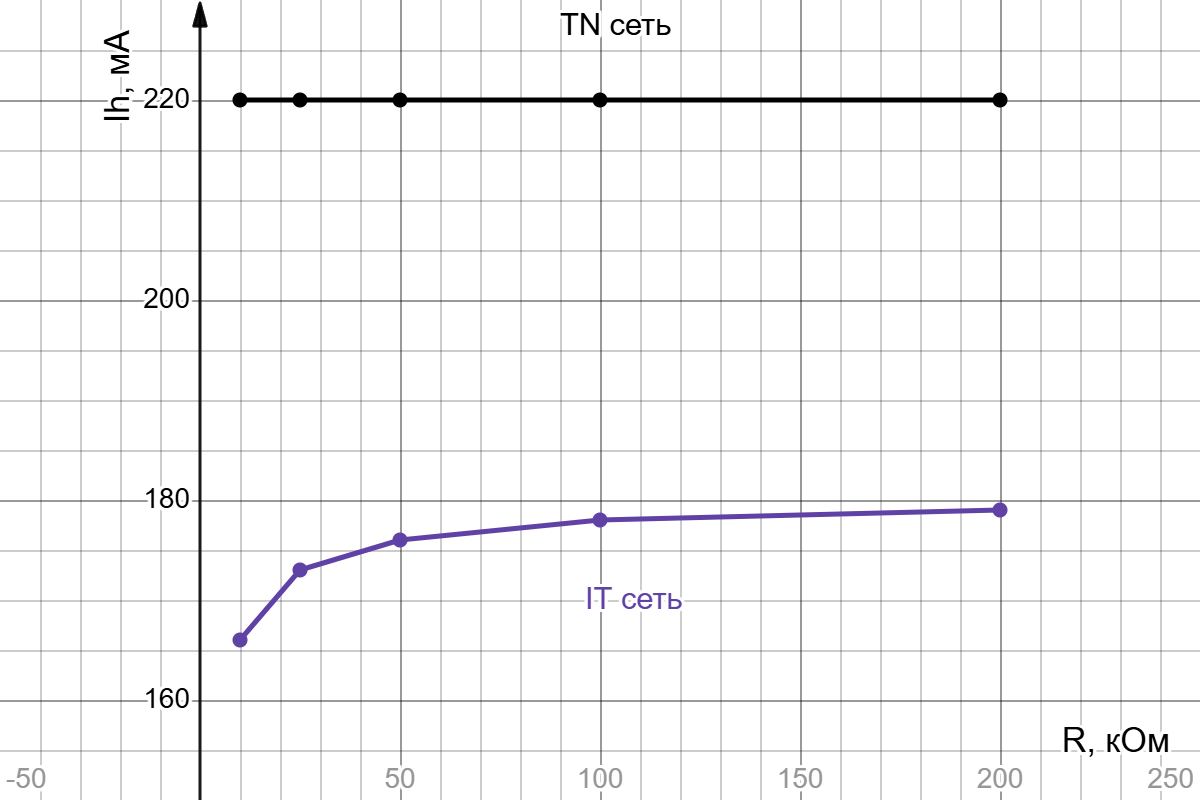
\includegraphics[width=\textwidth]{png/i(r).png}
		\captionof{figure}{Зависимость $I_h(R)$}
		\label{i(r)}
	\end{minipage}
	\begin{minipage}{.5\textwidth}
		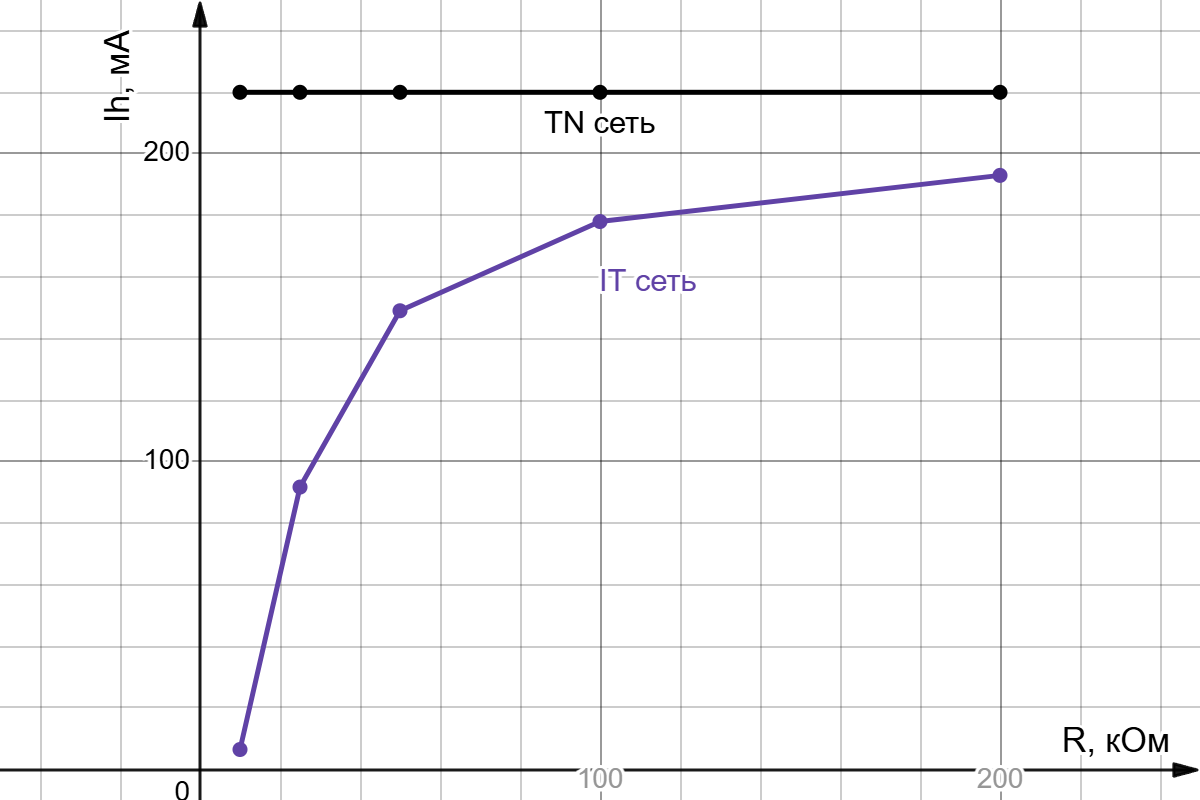
\includegraphics[width=\textwidth]{png/i(c).png}
		\captionof{figure}{Зависимость $I_h(C)$}
		\label{i(c)}
	\end{minipage}

	\newpage

	\section{Выводы}
	
	В ходе этой работы была проанализирована опасность прикосновения человека к токоведущим частям трёхфазной сети с номинальным фазным напряжением в 220\,В. Во многих случаях такое прикосновение несёт опасность для человека. 
	
	Можно отметить, что наименее опасным является прикосновение к нейтрали. В нормальном режиме она не находится под напряжением и никакой опасности не несёт. В аварийном режиме прикосновение к ней пропускает через человека ток, но его значение невелико и будет лишь ощутимо.
	
	Прикосновение к фазным проводам вне зависимости от общей исправности системы и этого конкретно провода опасно. Почти во всех случаях человек подвергается фибрилляционному току. В случае взятия за неисправный провод в сети с изолированной нейтралью человек подвергается неотпускающему току, что тоже несёт опасность, но значение такого тока меньше, чем фибрилляционного.

\end{document}
